\documentclass{beamer}

\usepackage[orientation=portrait,size=a0,scale=1.4]{beamerposter}
\mode<presentation>{\usetheme{ESO}}
\usepackage[utf8]{inputenc}
\usepackage{ragged2e}
\usepackage[font=small,justification=justified]{caption}
\usepackage{array,booktabs,tabularx}
\usepackage{grffile}
\usepackage{hyperref}

\usepackage[
    style=authoryear
]{biblatex}  % import biblatex for bibliography
\addbibresource{refs.bib} % include the file having references
\AtNextBibliography{\footnotesize}  % for smaller font of references
% \usepackage{lmodern} % Latin Modern fonts, fully scalable
% \usepackage{helvet}
% \renewcommand{\familydefault}{\sfdefault} % Set sans-serif as default font


\DeclareRobustCommand{\ion}[2]{\textup{#1\,\textsc{\textup{#2}}}}
\newcommand*\arcmin{\ensuremath{^\prime}}
\newcommand*\arcsec{\ensuremath{^{\prime\prime}}}



% \title[SBS\,0335-052E]{A $\sim$15 kpc outflow cone emanating from the compact starburst SBS\,0335-052E}
\title[SBS\,0335-052E]{Statistical signature of biconical outflows traced by HI and OVI}

% \author{E.~C.~Herenz$^1$, J.~M.~Cannon$^2$, J.~Inoue$^2$, M.~Hayes$^3$, C.~Moya-Sierralta$^4$, P.~Papaderos$^5$, and G.~Östlin$^3$}
\author{Sourav Das$^1$, Sayak Dutta$^1$, Sowgat Muzahid$^1$, MUSE GTO Consortium}

% \institute[]{$^1$ESO Fellow, Chile -- $^2$Macalester College, USA
%   -- $^3$Stockholm University, Sweden -- $^4$Pontificia Universidad
%   Cat\'{o}lica de Chile -- $^5$Institute of Astrophysics and Space
%   Sciences, Portugal}
\institute[]{$^1$Inter-University Centre for Astronomy \& Astrophysics, Post Bag 04, Pune, India 411007}


% \date{LymanRAS Online Workshop -- Jan 14, 2022}
\date{BBGB 2024}

\begin{document}

\begin{frame}
  \begin{columns}[c]
    \begin{column}{0.99\textwidth} \vspace{+0.3em}
      \begin{block}{Angular Distributions of Gas and Metals in the Circumgalactic       Medium: Insights into Galaxy Evolution}
        \large Understanding the angular distribution of gas and metals in the circumgalactic medium (CGM) offers critical insights into the gas flow processes that regulate galaxy evolution. Gas accretion is often hypothesized to occur preferentially along the disk plane, while metal-enriched winds are thought to outflow along the minor axis, following paths of least resistance. We present an observational study of the azimuthal dependence of gas and metals in the CGM of a statistically significant sample of low-redshift galaxies, leveraging UV absorption-line data obtained using HST/COS. Morphological parameters, such as the inclination angles and position angles, were derived by modeling galaxy light profiles using GALFIT on HST images. We find an enhanced HI covering fraction along both the major and minor axes within 1.5 $R_{\text{vir}}$, whereas the OVI covering fraction increases steadily as a function of azimuthal angle.
        % corresponding to cool accreting gas and the cool phase of outflows, respectively. In contrast, the elevated OVI covering fraction in the CGM along the minor axis points to warm-hot bipolar outflows.
        % Understanding the angular distribution of gas and metals in the circumgalactic medium (CGM) offers critical insights into the gas flow processes that regulate galaxy evolution. Gas accretion is often hypothesized to occur preferentially along the disk plane, while metal-enriched winds are thought to outflow along the minor axis, following paths of least resistance. We present an observational study of the azimuthal dependence of gas and metals in the CGM of a statistically significant sample of low-redshift galaxies, leveraging UV absorption-line data obtained using HST/COS. Morphological parameters, such as the inclination angles and position angles, were derived by modeling galaxy light profiles using GALFIT on HST images. We find an enhanced HI covering fraction along both the major and minor axes within 1.5 Rvir, whereas the OVI covering fraction increases steadily as a function of azimuthal angle.
        \end{block}
    \end{column}
  \end{columns}
  \vspace{0.5cm}
  \begin{columns}[T]
    \begin{column}{0.48\textwidth}
      \begin{beamercolorbox}[center,wd=\textwidth]{postercolumn}
        \begin{block}{HST Imaging and Spectroscopic Data} 
            The galaxy sample for this study is drawn from the catalog of nearly 6000 low $z$ galaxies compiled by \cite{dutta2023musequbes}, detected in the foregrounds of 190 UV-bright quasars with Hubble Space Telescope (HST) Cosmic Origins Spectrograph (COS) spectra. Using quasar coordinates, a cone search with a radius of 3 arcsec in the HST public archive identified 81 fields observed with the Advanced Camera for Surveys (ACS), Wide Field Camera 3 (WFC3), or Wide Field Planetary Camera 2 (WFPC2). These instruments provide high-resolution, diffraction-limited imaging with plate scales of 0.04–0.13 arcsec/pixel.
            
           We identified 42 images that contain 424 foreground galaxies within their fields of view, forming the foundation for our imaging and spectroscopic analysis.


          % \vspace{0.5cm}
          \begin{figure}
            \begin{minipage}{\textwidth}
              \centering
              % \includegraphics[width=\textwidth, trim=65 38 30 30,
              % clip=true]{./figs2021/plot_rgb_muse_inset_N0_7ktaper.pdf}
              % \\\vspace{1em}
              % \includegraphics[width=0.475\textwidth, trim=90 23 31 5,
              % clip=true]{./figs2021/plot_Ha_w_cont_21cm_notaper.pdf} 
              % \includegraphics[width=0.45\textwidth,trim=80 25 60
              % 0,clip=true]{./figs2021/hst_f656n_21cm_newdat.pdf}
              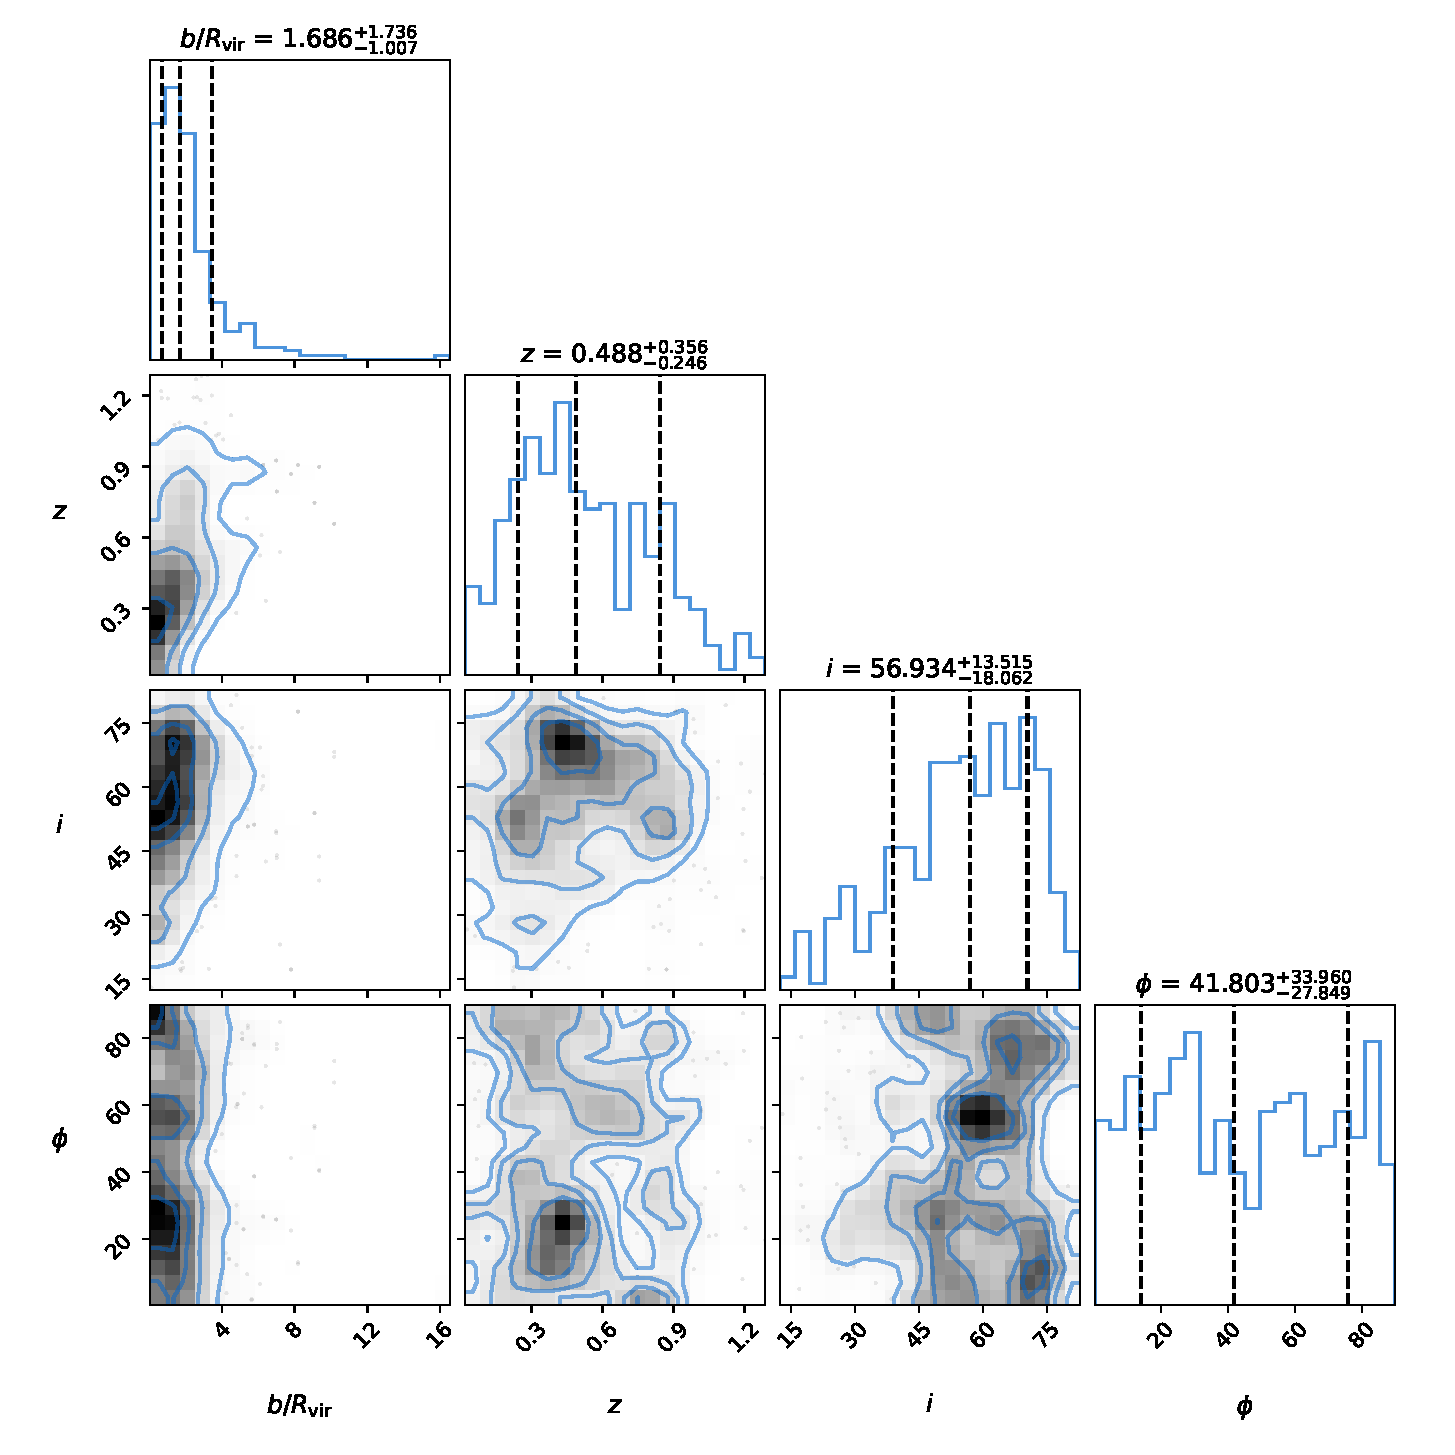
\includegraphics[width=0.9\textwidth]{./images/corner_plot.pdf}
              % \vspace{1em}
              \caption{Distributions and correlations of key galaxy parameters: impact parameter normalized by virial radius ($b/R_{\text{vir}}$), redshift ($z$), inclination angle ($i$), and azimuthal angle ($\phi$).}
              % \caption{\emph{Top:} 30h JVLA B-configuration
              %   observations of SBS 0335-052 system (red contours at
              %   $N_\text{HI}= \{0.7, 1.6, 2.8, 3.6, 5.4 \} \times
              %   10^{20}$\,cm$^{-2}$; 7k$\lambda$ tapered data; beam is
              %   15.9\arcsec{}$\times$14.7\arcsec{} oriented at
              %   66.4$^\circ$) overlaid on H$\alpha$ narrow-band from
              %   MUSE (log-stretch from 0 to
              %   1.25$\times10^{-15}$\,erg\,s$^{-1}$cm$^{-2}$) inset
              %   into a colour composite (grz from
              %   Pan-STARRS). \emph{Bottom left:} H$\alpha$ from MUSE
              %   ($t_\text{exp.}=1.5$\,h, cyclic colour map from 0 to
              %   $10^{-18}$ to $10^{-15}$\,erg\,s$^{-1}$cm$^{-2}$ with
              %   asinh-scaling; contours
              %   \(\text{SB}_{H\alpha}=\{0.75, 1.5, 2.5, 5, 12.5\}
              %   \times 10^{-18}\)\,erg\,s$^{-1}$cm$^{-2}$) with
              %   untapered HI 21cm from JVLA. \emph{Bottom right:}
              %   Untapered JVLA 21cm B-configuration observations (red
              %   contours; 6.1\arcsec{}$\times$6.1\arcsec{} beam at
              %   -23.6$^\circ$).  Contour levels represent
              %   $N_\text{HI} = \{6, 9, 11, 14, 18.5, 27.8\}\times
              %   10^{20}\,\text{cm}^{-2}$.  The background HST
              %   H$\alpha$ (FR656N) image is displayed with a cyclic
              %   asinh-stretch highlighting the bright emission near
              %   the super star clusters while also providing contrast
              %   for the filamentary loops in the NW.  }
              \label{fig:1}
            \end{minipage}
          \end{figure}

          \begin{figure}
            \begin{minipage}{0.4\textwidth}
              \centering
              % \includegraphics[width=\textwidth, trim=65 38 30 30,
              % clip=true]{./figs2021/plot_rgb_muse_inset_N0_7ktaper.pdf}
              % \\\vspace{1em}
              % \includegraphics[width=0.475\textwidth, trim=90 23 31 5,
              % clip=true]{./figs2021/plot_Ha_w_cont_21cm_notaper.pdf} 
              % \includegraphics[width=0.45\textwidth,trim=80 25 60
              % 0,clip=true]{./figs2021/hst_f656n_21cm_newdat.pdf}
              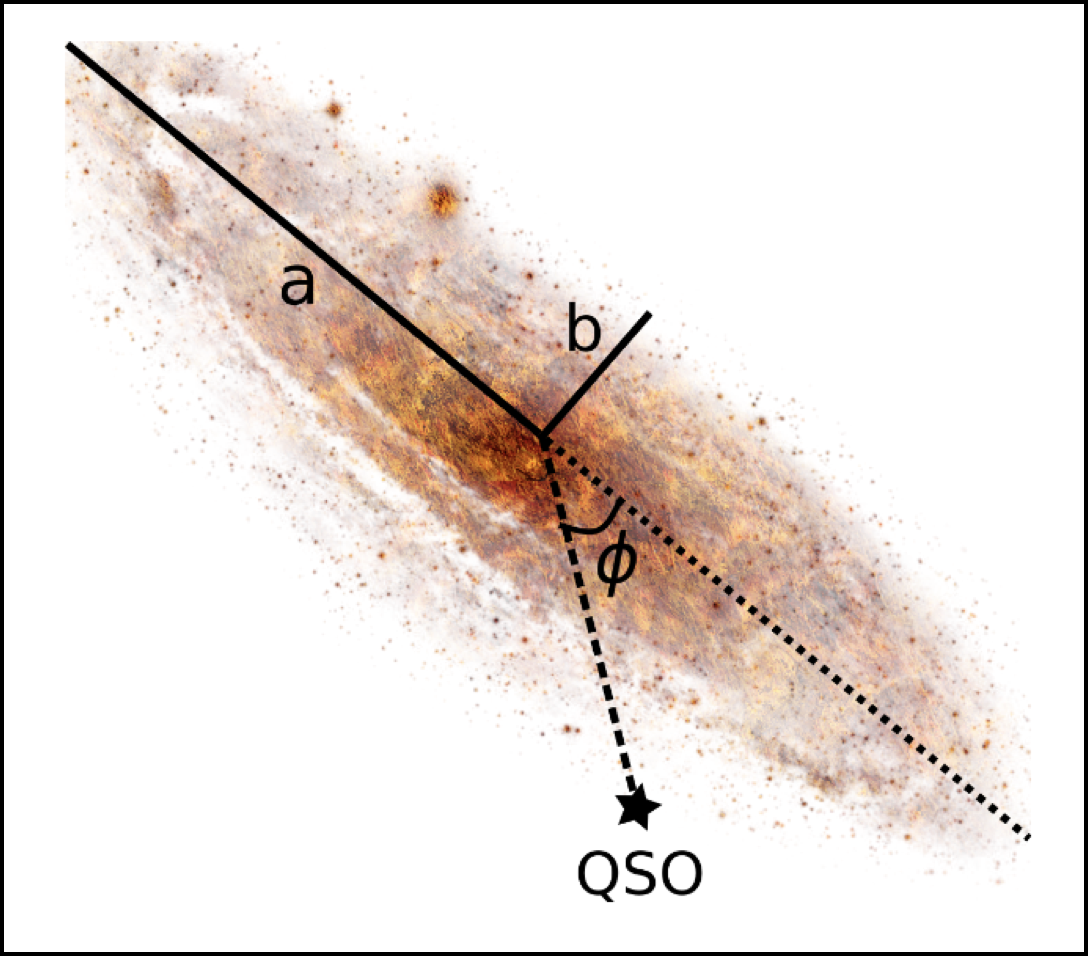
\includegraphics[width=0.8\textwidth, trim=12 10 10 10, clip=true]{./images/az_angle}
              % \vspace{1em}
              \caption{Schematic representation of semi-minor axis ($b$), semi-major axis ($a$), and azimuthal angle ($\phi$) of a galaxy with respect to a QSO.}
              \label{fig:2}
            \end{minipage}%
            \hspace{0.02\textwidth}
            \begin{minipage}{0.5\textwidth}
              \centering
              % \includegraphics[width=\textwidth, trim=65 38 30 30,
              % clip=true]{./figs2021/plot_rgb_muse_inset_N0_7ktaper.pdf}
              % \\\vspace{1em}
              % \includegraphics[width=0.475\textwidth, trim=90 23 31 5,
              % clip=true]{./figs2021/plot_Ha_w_cont_21cm_notaper.pdf} 
              % \includegraphics[width=0.45\textwidth,trim=80 25 60
              % 0,clip=true]{./figs2021/hst_f656n_21cm_newdat.pdf}
              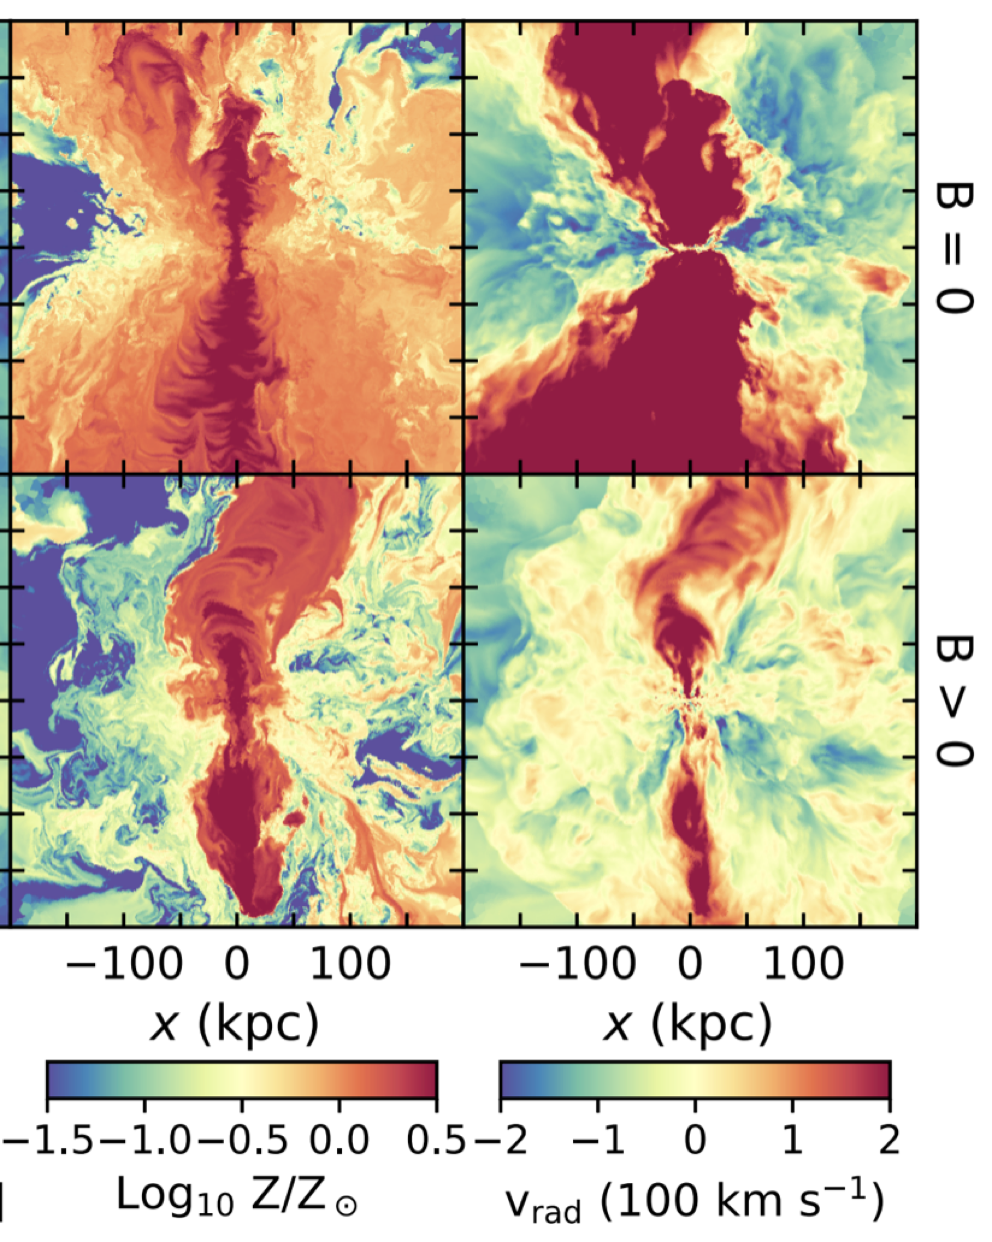
\includegraphics[width=0.5\textwidth]{./images/voort_simulation}
              % \vspace{1em}
              \caption{400 $\times$ 400 kpc$^{2}$ images of the gas in and around an edge-on Milky Way-mass galaxy at $z=0$ in a simulation without magnetic fields (top panels) and with magnetic fields (bottom panels) (\cite{2021MNRAS.501.4888V}). }
              \label{fig:3}
            \end{minipage}
          \end{figure}
          %In Figure 3, Metallicity is highest along the polar direction in both cases, while other regions of the CGM are more enriched without magnetic fields, indicating more efficient gas mixing. Radial velocity exhibits strong temporal variability but generally shows more confined outflows when magnetic fields are present (\cite{2021MNRAS.501.4888V}).

        \end{block}\vspace{-0.5cm}
      \end{beamercolorbox}
    \end{column}
    \begin{column}{0.48\textwidth}
      \begin{block}{Galaxy light profile fitting using GALFIT}
        We used GALFIT (\cite{2010AJ....139.2097P}), a non-linear least-squares fitting software, to model the light profiles of galaxies in our sample and extract morphological parameters like position angle and axis ratio. A single-component Sérsic profile was sufficient for our purpose, focusing on obtaining these parameters rather than perfect residuals. A Python wrapper was developed for batch fitting, automating the process for hundreds of galaxies with randomized initial guesses. Median values of converged runs ensured reliable results.
        \begin{figure}
          % \centering \includegraphics[width=0.77\textwidth, trim=95 25
          % 0 0, clip=true]{./figs2021/plot_velfield_experiment.pdf} \vspace{1cm}
          % \caption{Velocity field of the ionised gas as derived from
          %   the MUSE observations.  The major- and minor-axes from HI
          %   kinematics are delineated as dash-doted and dotted lines,
          %   respectively.}
          % \label{fig:2}
          \centering
          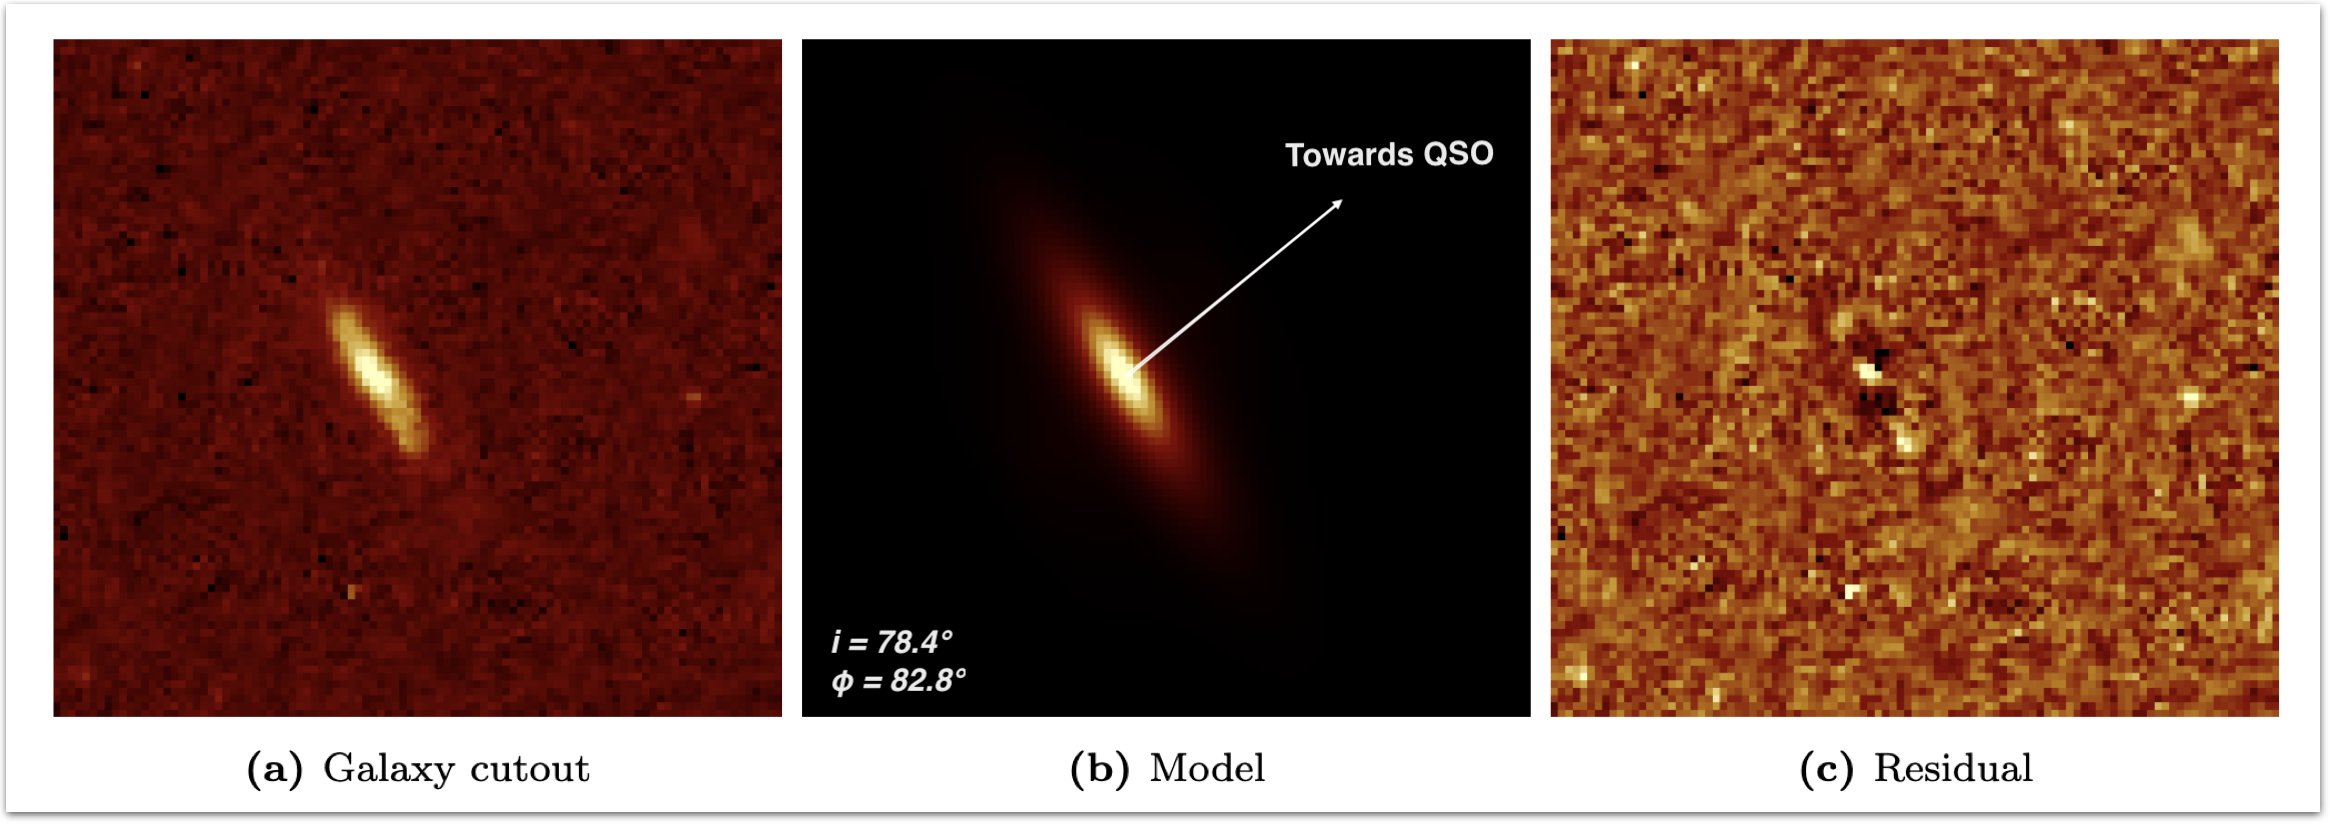
\includegraphics[width=\textwidth]{./images/galfit_model}
          \caption{Output FITS file from GALFIT for one of the galaxies in our sample, showing the galaxy cutout, the fitted model, and the residual.}
        \end{figure}
      \end{block}
      \vspace{1.1cm}
      \begin{block}{Covering Fraction Analysis: HI and OVI}
        We performed a covering fraction analysis to study the distribution of HI and OVI in our sample. Using COS spectra, we calculated the covering fractions of these species across different bins of the azimuthal angle, $\phi$. The azimuthal angle bins are defined to investigate the spatial distribution of gas relative to the galaxy's major axis. For HI, the covering fraction provides insights into the extent of cool, neutral gas, while the OVI measurements trace hotter, more ionized gas in the CGM. Our analysis reveals trends in the covering fraction that are sensitive to $\phi$, suggesting distinct physical and dynamical processes governing the HI and OVI distributions in the CGM.
        
%          \vspaceo{-0.3cm}
          \begin{figure}
            \centering 
            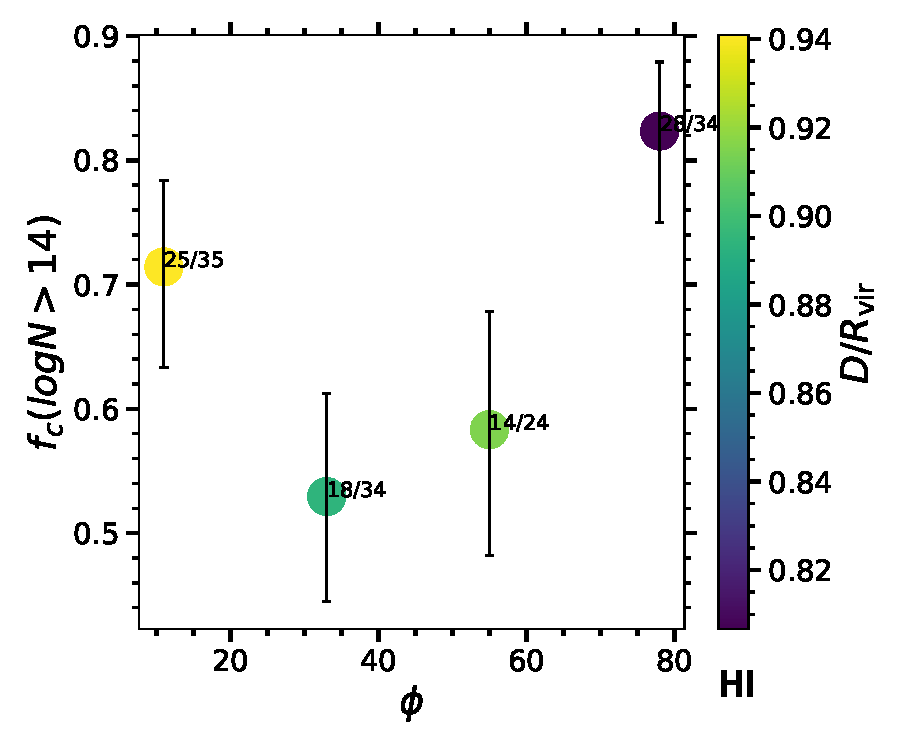
\includegraphics[width=0.49\textwidth]{./images/phi_dep_dnorm_lt1.5.pdf}
            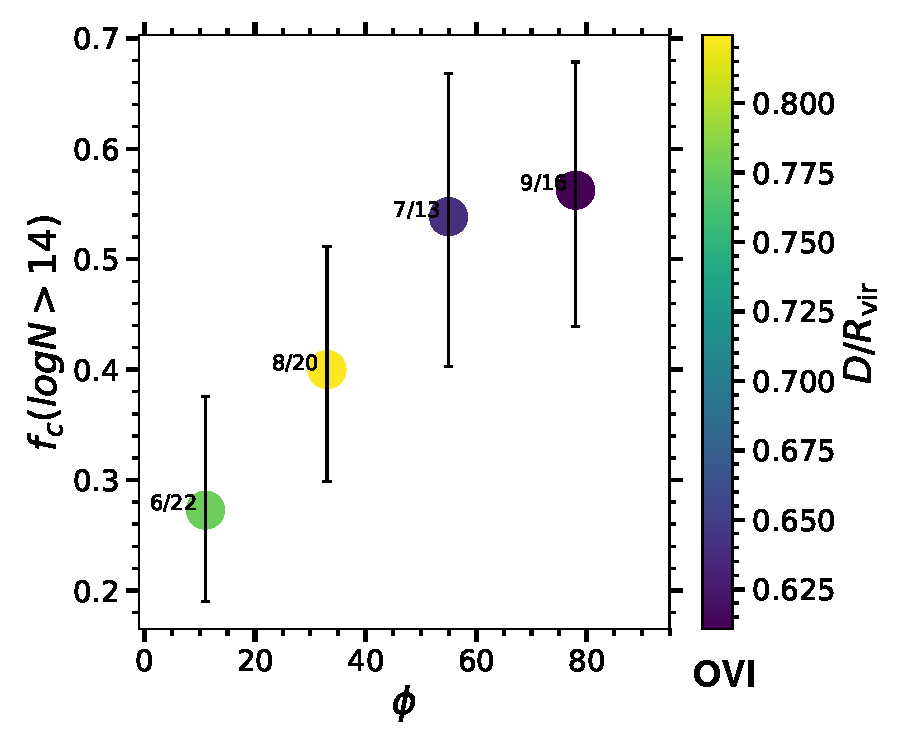
\includegraphics[width=0.49\textwidth]{./images/phi_dep_dnorm_lt1.0.pdf}
            \begin{picture}(0,0) % Start overlay for annotations
                \put(-750,100){\small \textbf{HI}}
                \put(-250,100){\small \textbf{OVI}}
            \end{picture}
            \caption{Covering fraction of HI (left) and OVI (right) as a function of azimuthal angle, color-coded by the impact parameter normalized to the virial radius.}
            \label{fig:model}
          \end{figure}
        In figure \ref{fig:3}, metallicity is highest along the polar direction in both cases, while other regions of the CGM are more enriched without magnetic fields, indicating more efficient gas mixing. Radial velocity exhibits strong temporal variability but generally shows more confined outflows when magnetic fields are present (\cite{2021MNRAS.501.4888V}).
        \end{block}
    \end{column}
  \end{columns}
  % \vspace{0.5cm}
  \begin{columns}
    \begin{column}{0.99\textwidth}
      \begin{block}{Conclusions}
          We find an enhanced HI covering fraction along both the major and minor axes within 1.5 $R_{\text{vir}}$, corresponding to cool accreting gas and the cool phase of outflows, respectively. In contrast, the elevated OVI covering fraction in the CGM along the minor axis points to warm-hot bipolar outflows.
      \end{block}
    \end{column}
  \end{columns}
  % \vspace{0.5cm}
  \begin{columns}
    \begin{column}{0.99\textwidth}
      \begin{block}{References}
        % \scriptsize
        \printbibliography[title = {References}]
         \noindent \footnotesize{Das, Sourav et al. (in prep)} \\
        % \printbibliography[title = {References}]
      \end{block}
    \end{column}
  \end{columns}
\end{frame}


\end{document}


%%% Local Variables:
%%% mode: latex
%%% TeX-master: t
%%% End:
